 %
\documentclass[11pt]{article}

\usepackage[utf8]{inputenc}
\usepackage{amsmath}
\usepackage{amsthm}
\usepackage{amssymb}
\usepackage{mathabx} 
\usepackage{graphicx}
\usepackage{color} 
\usepackage{setspace} 
\usepackage{rotating}
\usepackage{natbib}
\usepackage{multirow}
\usepackage{xspace}
\usepackage{lscape}
%\usepackage{cite}
\usepackage{xr}
\usepackage{bbm}
\usepackage[normalem]{ulem}
\usepackage{newtxtext}
\usepackage{listings}
\usepackage{amssymb}
\usepackage[linesnumbered,lined,boxed,commentsnumbered,noend,ruled,vlined]{algorithm2e}

\usepackage{datetime}
\newdateformat{monthyeardate}{%
  \monthname[\THEMONTH], \THEYEAR}


\usepackage[labelfont=bf,labelsep=period,justification=raggedright]{caption}

\usepackage{hyperref}
\urlstyle{rm}
\hypersetup{
  colorlinks,
  urlcolor=blue,
  linkcolor=black,
  citecolor=black
}

% Text layout
\oddsidemargin 0in
\evensidemargin 0in
\topmargin -.5in
\textwidth 6.5in
\textheight 9in

\externaldocument{mcref}


% Remove brackets from numbering in List of References
\makeatletter
\renewcommand{\@biblabel}[1]{\quad#1.}
\newcommand{\smallCom}[1]{\marginpar{\tiny{#1}}}
\newcommand{\vect}[1]{\boldsymbol{\mathbf{#1}}}
\newcommand{\ld}{\mathcal{L}}
\newcommand{\ignore}[1]{}
\newcommand{\mcref}{\textsc{McRef}\xspace}
\newcommand{\E}{\mathbb{E}}
\newcommand{\X}{\vect{X}}
\newcommand{\M}{\mathcal{M}}
\newcommand{\Tr}{\mathcal{T}}
\newcommand{\B}{\vect{B}}
\newcommand{\Y}{\vect{Y}}
\newcommand{\G}{\vect{G}}
\newcommand{\T}{\vect{\Theta}}
\newcommand{\I}{\mathbb{I}}
\newcommand{\Ip}{\mathcal{I}(p,l)}
\newcommand{\Ib}{\mathcal{I}(b,l)}
\newcommand{\GT}{\G\T}
\newcommand{\Mref}{\M_{ref}}
\newcommand{\Mhyp}{\M_{hyp}}
\newcommand{\Mnull}{\M_{null}}
\newcommand{\Pref}{\widetilde{P}}
\newcommand{\rbf}{\text{BF}}
%\newcommand{\hbf}{\text{BF}}
\newcommand{\Om}{\Omega}
\newcommand{\GTref}{\widetilde{\GT}}
\newcommand{\Gref}{\widetilde{\G}}
\newcommand{\Tref}{\widetilde{\T}}
\newcommand{\1}{\mathbbm{1}}
\newcommand{\Z}{\vect{Z}}
\newcommand{\Zref}{\widetilde{\Z}}
\newcommand{\Omref}{\widet	ilde{\Om}}
\newcommand{\Fext}{F_{Z}}
\newcommand{\troot}{\theta_{root}}
\newcommand{\Gc}{\G_c}
\newcommand{\Gm}{\G_m}
\newcommand{\gp}{G-PhoCS }
\def\comb{\rotatebox[origin=c]{90}{$\exists$}}
\newcommand{\Mcomb}{\M_{\comb}}
\newcommand{\Gcomb}{\G_{\comb}}
\newcommand{\Tcomb}{\T_{\comb}}
\newcommand{\tmin}{\tau_{\text{min}}}
% Two lines from genres
\def\@cite#1#2{(#1\if@tempswa , #2\fi)}
\def\@biblabel#1{}



% Default fixed font does not support bold face
\DeclareFixedFont{\ttb}{T1}{txtt}{bx}{n}{10} % for bold
\DeclareFixedFont{\ttm}{T1}{txtt}{m}{n}{10}  % for normal

% Custom colors
\usepackage{color}
\definecolor{deepblue}{rgb}{0,0,0.5}
\definecolor{deepred}{rgb}{0.6,0,0}
\definecolor{deepgreen}{rgb}{0,0.5,0}

\usepackage{listings}

% Python style for highlighting
\newcommand\pythonstyle{\lstset{
language=Python,
basicstyle=\ttm,
otherkeywords={self},             % Add keywords here
keywordstyle=\ttb\color{deepblue},
emph={recursive_num_coals,recursive_coal_stats},% Custom highlighting
emphstyle=\ttb\color{deepred},    % Custom highlighting style
stringstyle=\color{deepgreen},
frame=tb,                         % Any extra options here
showstringspaces=false            % 
}}


% Python environment
\lstnewenvironment{python}[1][]
{
\pythonstyle
\lstset{#1}
}
{}

% Python for external files
\newcommand\pythonexternal[2][]{{
\pythonstyle
\lstinputlisting[#1]{#2}}}

% Python for inline
\newcommand\pythoninline[1]{{\pythonstyle\lstinline!#1!}}

\newenvironment{tightcenter}{%
  \setlength\topsep{0pt}
  \setlength\parskip{0pt}
  \begin{center}
}{%
  \end{center}
}

\graphicspath{ {images/} }

\author{Ron Visbord}
% \newcommand{\smallCom}[1]{\marginpar{\tiny{#1}}}

\begin{document}


\begin{titlepage}
	\centering
	
\includegraphics[width=0.4\textwidth]{IDC_logo}\par\vspace{2cm}
	{\huge The Interdiciplinary Center, Herzliya \par}
	{\Large Efi Arazi School of Computer Science \par}
	{\Large M.Sc. Program - Research Track \par}
	
	\vspace{1cm}
	
	\vspace{1.5cm}
	{\Huge A New Bayesian Method for Comparing Demographic Models \par}
	\vspace{3cm}
	{\large by\par}
	{\large\bfseries Visbord Ron\par}
	
	\vspace{2cm}
	{M.Sc. dissertation, submitted in partial fulfillment of the requirements\par}
	{for the M.Sc. degree, research track, School of Computer Science\par}
	{The Interdisciplinary Center, Herzliya}
	
	\vfill
	
	% Bottom of the page
	{\large \monthyeardate\today \par}
	
\end{titlepage}

\newpage

This work was carried out under the supervision of Dr. Ilan Gronau from the Efi Arazi School of Computer Science, The Interdiciplinary Center, Herzliya.

\newpage

\section*{Abstract}
High throughput sequencing has greatly improved our ability to investigate the evolutionary history of species using detailed demographic models. A popular approach for inferring parameters in these demographic models is by sampling genealogical histories at many short unlinked loci using a Markov Chain Monte Carlo algorithm. The use of explicit coalescent models by these methods makes them powerful for inferring demographic parameters, but they are limited in their ability to assess the fit of the inferred model to data. The purpose of this research is to examine a new approach, based on Relative Bayes Factors, for using genealogy samples to compare different evolutionary hypotheses. 


\newpage

\tableofcontents

\newpage



















%%%%%%%%%%%%%%%%%%%%%%%%%%%%%%%%%%%%%%%%%%%%%%%%%%%%%%%%%%%%%%%%%%%%%%%%%%%%%%%%%
%%%%%%%%%%%%%%%%%%%%%%%%%%%% HERE STARTETH THE PAPER %%%%%%%%%%%%%%%%%%%%%%%%%%%%
%%%%%%%%%%%%%%%%%%%%%%%%%%%%%%%%%%%%%%%%%%%%%%%%%%%%%%%%%%%%%%%%%%%%%%%%%%%%%%%%%



\section{Introduction}

In recent years, advances in high throughput DNA sequencing have made it easy to sequence large amounts of genomes of individuals from closely related species. This allows evolutionary biologists to examine the evolution of recently diverged species by employing data-intensive computational methods and statistical models.
%
Typically, an evolutionary biologist, having obtained multiple aligned genome sequences from relative species or populations, would like to recreate the evolutionary history of the sequenced individuals. This evolutionary history includes a series of population splits, population ancestry and divergences, population size changes and post-divergence gene flow.\\
%
The job of retracing this evolutionary history may be viewed as two seperate tasks; First, one must find the phylogenetic model structure. This is a tree-like graph which represents the ancestral relation between all relevant populations, as well as any migration bands between populations. This task is often referred to as \textbf{Model selection}. Second, having obtained the model structure, one must find the phylogenetic model parameters. These are the specific parameter values or distributions of the model, such as population divergence times, population sizes and migration rates. This is the task of \textbf{Parameter Inference}.\\
%
Many existing popular methods perform parameters inference (task II) by assuming the evolutionary structure and performing bayesian inference on model parameters [TODO - reference methods]. These methods are effective because ??? [TODO - succintly explain why these methods are effective]. However, they cannot effectively assess the fit of the sequence data to the assumed model structure because ??? [TODO - explain this claim].
%
Alternative methods for directly assessing the fit of sequence data to some phylogenetic model exist [TODO - reference methods s.a. harmonic mean...] but these are known to have high variance or be too cpu-intensive [TODO - rewrite previous sentence with proper explanation].
%
This leaves us with no robust tools for selecting the model structure which best fits the sequence data.\\
%
The goal of our research is thus to \textbf{utilize bayesian parameter inference methods to perform robust model selection}.
%
We accomplish this by introducing the concept of \textbf{Reference Models}, which are generic/base-line/bridging phylogenetic models used to asses model fit to data within a specific context, allowing us to choose between competing model candidates.
%
We will start by overviewing existing work in the field and laying down the background of common notations for phylogenetic models and parameter inference.
%
We will then formally develop from scratch the concept of reference models, how the relate to phylogenetic population models, how they are used for model comparison criteria, and [maybe] why they are advantagous over existing methods. 
%
We will then explain in detail our implementation of reference-model-based model selection, nicknamed \textbf{McRef}, based on the \gp parameter-inference framework.
%
Finally we will share empirical results from our model-comparison experiments, showcasing the advantages and limitations of our implementation.

\subsection{Other Relevant Work}

Discuss structure+parameter inference methods here - 

\begin{itemize}
\item general methods (non bayesian)for history reconstruction. what are the drawbacks in "likelihood-based" approaches?

\item importance-sampling based

\item thermodynamic stuff for improving harmonic-mean (hopefully these methhods can also be applied on mcref)

\end{itemize}

\subsection{Unused leftovers from previous introduction}

\begin{itemize}
\item  Structure inference is all about choosing the evolutionary model which best fits the genom data. ...sometimes from scratch by searching the model/tree space (reference - https://www.nature.com/articles/nmeth.4285) and sometimes by discriminating candidates (newton-raftery, Lartillot N \& Philippe)
\item  overview of model-selection: www.webpages.uidaho.edu\/\~jacks\/Sullivan\&Joyce2005.pdf

\end{itemize}


\section{Background}


Demography inference methods typically take in aligned sequence data $X$ from a collection of individuals originating from closely related populations and a parameterized demographic model $\M$, and they infer
values of parameters $\T$ in that model. Bayesian methods achieve this by assuming some prior distribution on the model parameters $P(\T|\M)$ and sampling parameter values from an approximate posterior distribution $P(\T|\M, X)$. Because the joint probability distribution $P(X, \T|\M)$ cannot be efficiently computed, this task is often done by introducing local genealogies $G$ to the model, such that the probability $P(X , G, \T|\M)$ can be efficiently and accurately computed, and employing a Monte-Carlo Markov-Chain 1 (MCMC) sampling algorithm for $G$ and $\T$, e.g. IMa 2 , BP\&P 3 , and \gp 4. 
%
Sampling by MCMC guarantees that $\T$ \& $G$ will be sampled from a probability distribution approximating the posterior - $P(\T, G|X , \M)$. From this distribution one can extract approximate posterior means and credible intervals for all demographic parameters.

\gp is one such Bayesian demography inference method. Given sequence data, i.e. a small collection of unphased genomes at tens of thousands of short unlinked neutrally evolving loci , and given a population phylogeny model, \gp infers parameters $\T$ such as population divergence times $\tau$, ancestral population sizes $\theta$ and rates of post-divergence gene flow $m$. This is accomplished using MCMC sampling of local genealogies jointly with model parameters according to an approximate posterior distribution for full Bayesian inference.

\begin{figure}[h]
\centering
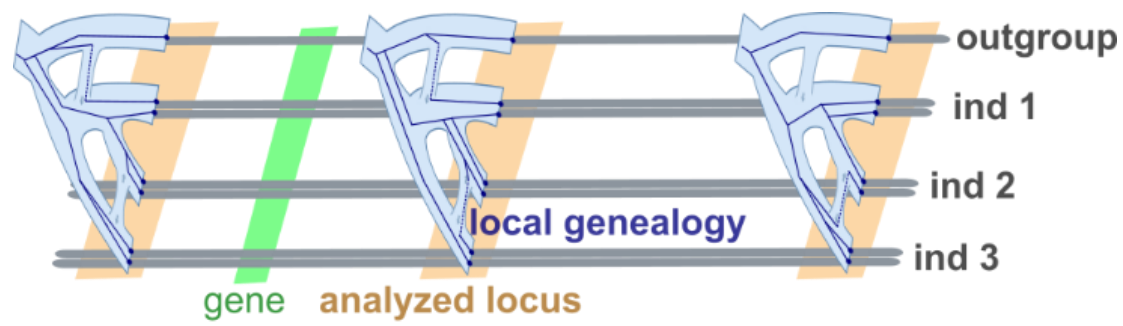
\includegraphics[width=0.8\textwidth]
{multiple_loci_across_sequence}
\caption{CAPTION CAPTION CAPTION}
\label{fig:clade_collapse_AB}
\end{figure}

In each iteration \gp proposes a new instace of $G, \T$ and decides whether to accept or reject the new proposal based on the ratio between likelihoods of the current instance and proposed instance. \gp assumes no recombination events within a locus, therefore the likelihood is a product across loci. Equation \ref{eq:likelihood} shows the likelihood calculation used by \gp
%
\begin{equation}\label{eq:likelihood}
 P(\X,\G,\T|\M) ~=~ P(\T|\M) P(\G|\M,\T) P(\X|\G) ~=~ P(\T|\M) \prod_l P(\G_l|\M,\T) P(\X_l|\G_l).
\end{equation}

Where $P(\T|\M)$ is the prior probability of model parameters to take current values, $P(\G_l|\M,\T)$ is the probability of logal genealogy $G_l$ given the model parameters, calculated under the Kingman Coalescent model, with special regard to migration events, and $P(\X_l|\G_l)$ is the local dna data likelihood given locus $G_l$.

\subsection{The Model Comparison problem}
More fundamental in the field of computational biology is the model comparison problem. \textbf{The model comparison problem aims to compare the fit to sequence data between a collection of structural models}. Models in this case are phylogenetic topologies, also known as population or demographic models. An example Model-Comparison question would be –\\
% 
\begin{tightcenter}{\textit{“Given sequence data $X$ of samples from
relative populations, which of the candidate phylogenetic topologies $\M$ best fits the data?“}}
\end{tightcenter}
\begin{figure}[h]
\centering
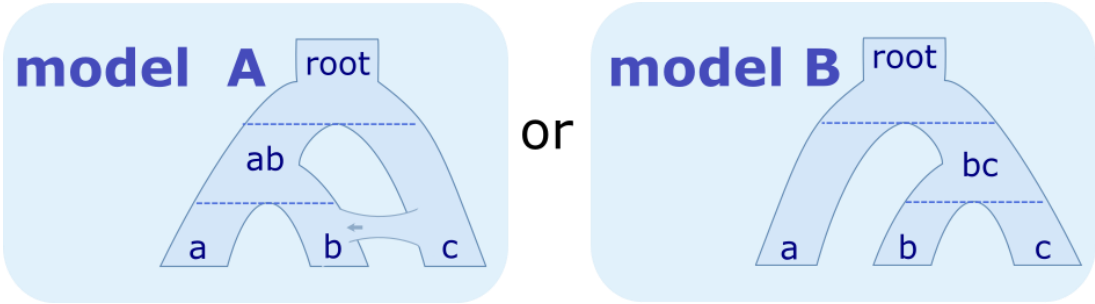
\includegraphics[width=0.8\textwidth]
{model_A__OR__model_b}
\caption{CAPTION CAPTION!}
\label{fig:model_A__OR__model_b}
\end{figure}

The Model Comparison Problem makes a distinction between structural components of model $\M$ (tree topology, migration bands, parameter priors) and parameter values $\T$ (specific migration rates, divergence times and population sizes). Model Comparison aims to compare different ‘model structures’.
%
Existing demography inference methods, such as \textcolor{red}{ Research 1, Paper 2 and Implementation 3}, don’t directly calculate likelihood - $P(X|\M)$, with or without parameters $\T$. The consequence is that researchers are unable to efficiently test many model hypotheses to explain the sample DNA data and tackle Model Comparison.
%
In this study, building upon the \gp demography inference method and MCMC sampler, we develop the theoretical framework for a robust model-comparison scheme, and implement a method to compare multiple models and their fit to the data, this without analytically calculating $P(X|\M)$.

We bear in mind that in most cases researchers are interested only in qualitative claims about the structure
of the model and not in qualitative claims about specific parameter values. To keep our method as
general as possible, the comparison algorithm we present receives no parameters $\T$ and will thus
output a result pertaining only to the topology of the model. This will allow us to test \textit{structural
hypotheses} by integrating over parameter values.

\subsection{An attempt – Standard Harmonic Mean}
One approach to model-comparison is to directly estimate the likelihood of the two candidate models, $P(X|\M_1)$  and  $P(X|\M_2)$. This is hard to analytically compute as $X$ and $M$ are only remotely related ,via $G$ and $\T$. One approach around this is the standard harmonic method. Defining $G\T$ as a joint random-variable of the genealogies and model parameters, we have - 

\begin{small}
\begin{align}
\mathbf{ HM(\M) ~:=~ \frac{1}{P(X|\M)} } ~&=~ \int \frac{P(G\T|\M)}{P(X|\M)} dG\T ~=~ \int \frac{P(G\T|\M)P(X,G\T|\M)}{P(X,G\T|\M)P(X|\M)}   dG\T \notag \\ 
%
&=~ \int \frac{P(G\T|X,\M)}{P(X|G\T)} dG\T ~=~ \mathbf{\E_{G\T|X,\M}\bigg[\frac{1}{P(X|G)}\bigg]} ~. 
\label{eq:harmonic_mean_estimator}
\end{align}
\end{small}

The last expression of equation \ref{eq:harmonic_mean_estimator} can be approximated using n MCMC samples of $\frac{1}{P(X|G)}$ from the posterior distribution $[G \T|X, \M]$ and calculating their mean. This approach fits naturally within the existing \gp framework for demography inference. However, since $\frac{1}{P(X|G)}$ is a random variable with very high variance (potentially unbounded when $G$ is distributed according to- $[G\T|X, \M]$ ), calculating its expectation is difficult and likely requires too large a number of samples.


\subsection{Our suggestion – Relative Bayes Factors}
...Explain McRef in high level terms and promise further explanation in main body...


\begin{figure}[h]
\centering
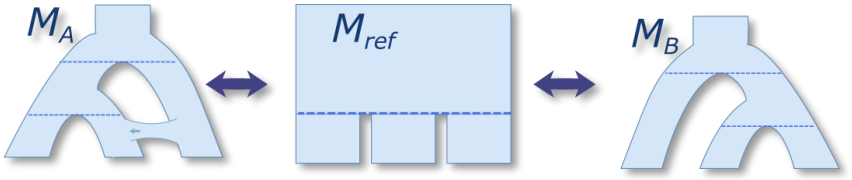
\includegraphics[width=0.8\textwidth]
{A_vs_B_via_ref}
\caption{To caption, or not to caption?}
\label{fig:model_A__OR__model_b}
\end{figure}



\newpage


\section{Preliminaries: demographic models and Bayesian inference}

\section{Methods}

\newpage

\section{Calculations Schema}

\subsection{The Computational Objective}

Consider formula (\ref{eq:rbf}) for calculating the Bayes Factor of model $M$ relative to $\Mref$:
%
%
\begin{equation}
 \frac{1}{\rbf(\M:\Mref|\X)}  ~~\approx~~ \frac{1}{N} \sum_{i=1}^{N}\frac{\Pref(\GT^{(i)}|\Mref) }{P(\GT^{(i)}|\M)} ~ 
\end{equation}

Since the denominator $P(\GT^{(i)}|\M)$ is constantly calculated by \gp in the MCMC process, what remains for mcref to calculate in order to estimate the Bayes Factor is the model pairing conditional $\Pref(\GT^{(i)}|\Mref)$. This is composed of hidden variable likelihoods and the genealogy likelihood over the reference model. See equations $(\ref{eq:pref_null})$, $(\ref{eq:pref_mig})$ and $(\ref{eq:rbf_comb_nomig})$ for examples of realizations of this formula for different reference models. The following chapter addresses efficiently calculating the \textbf{genealogy likelihood}, as it is the main component making up the model pairing conditional and represents the bulk of our computational challenge.\\

\subsection{Constructing a Reference Model}  \label{Constructing a Reference Model}


Every demographic model $\M$ has a variety of compatible reference models, which we would like to consider. A compatible reference model $\Mref$ may be obtained from the hypothesis model $\M$ by applying the following three-step process:

\begin{enumerate}
\item First, \textbf{choose a subtree} of the population phylogeny of $\M$. The subtree is associated with the population $p$ at its root. 

\item Then \textbf{collapse the subtree} using one of the structural collapse operations we introduce here. Generarlly speaking, \textit{collapsing} is the act of merging the populations of a subtree into a unified population. We describe two structural types of collapse operations; 

\textit{Clade-Collapse} is the operation of merging all the populations in a subtree rooted at $p$ into a single population denoted $clade(p)$. This new population will contain the portion of the genealogies previously located inside the subtree rooted at $p$ (see figure $\ref{fig:clade_collapse_AB}$). 

Similiarly, \textit{Comb-Collapse} is the operation of merging populations of a subtree, while perserving its leaves up to the comb-age. This operation will be detailed later.


\item Finally, \textbf{map the hidden parameters} of $\M$ onto parameters of $\Mref$ to define the model pairing conditional $\Pref$ (see section \textcolor{red}{ASDF}).
\end{enumerate}
%
\begin{figure}[h]
\centering
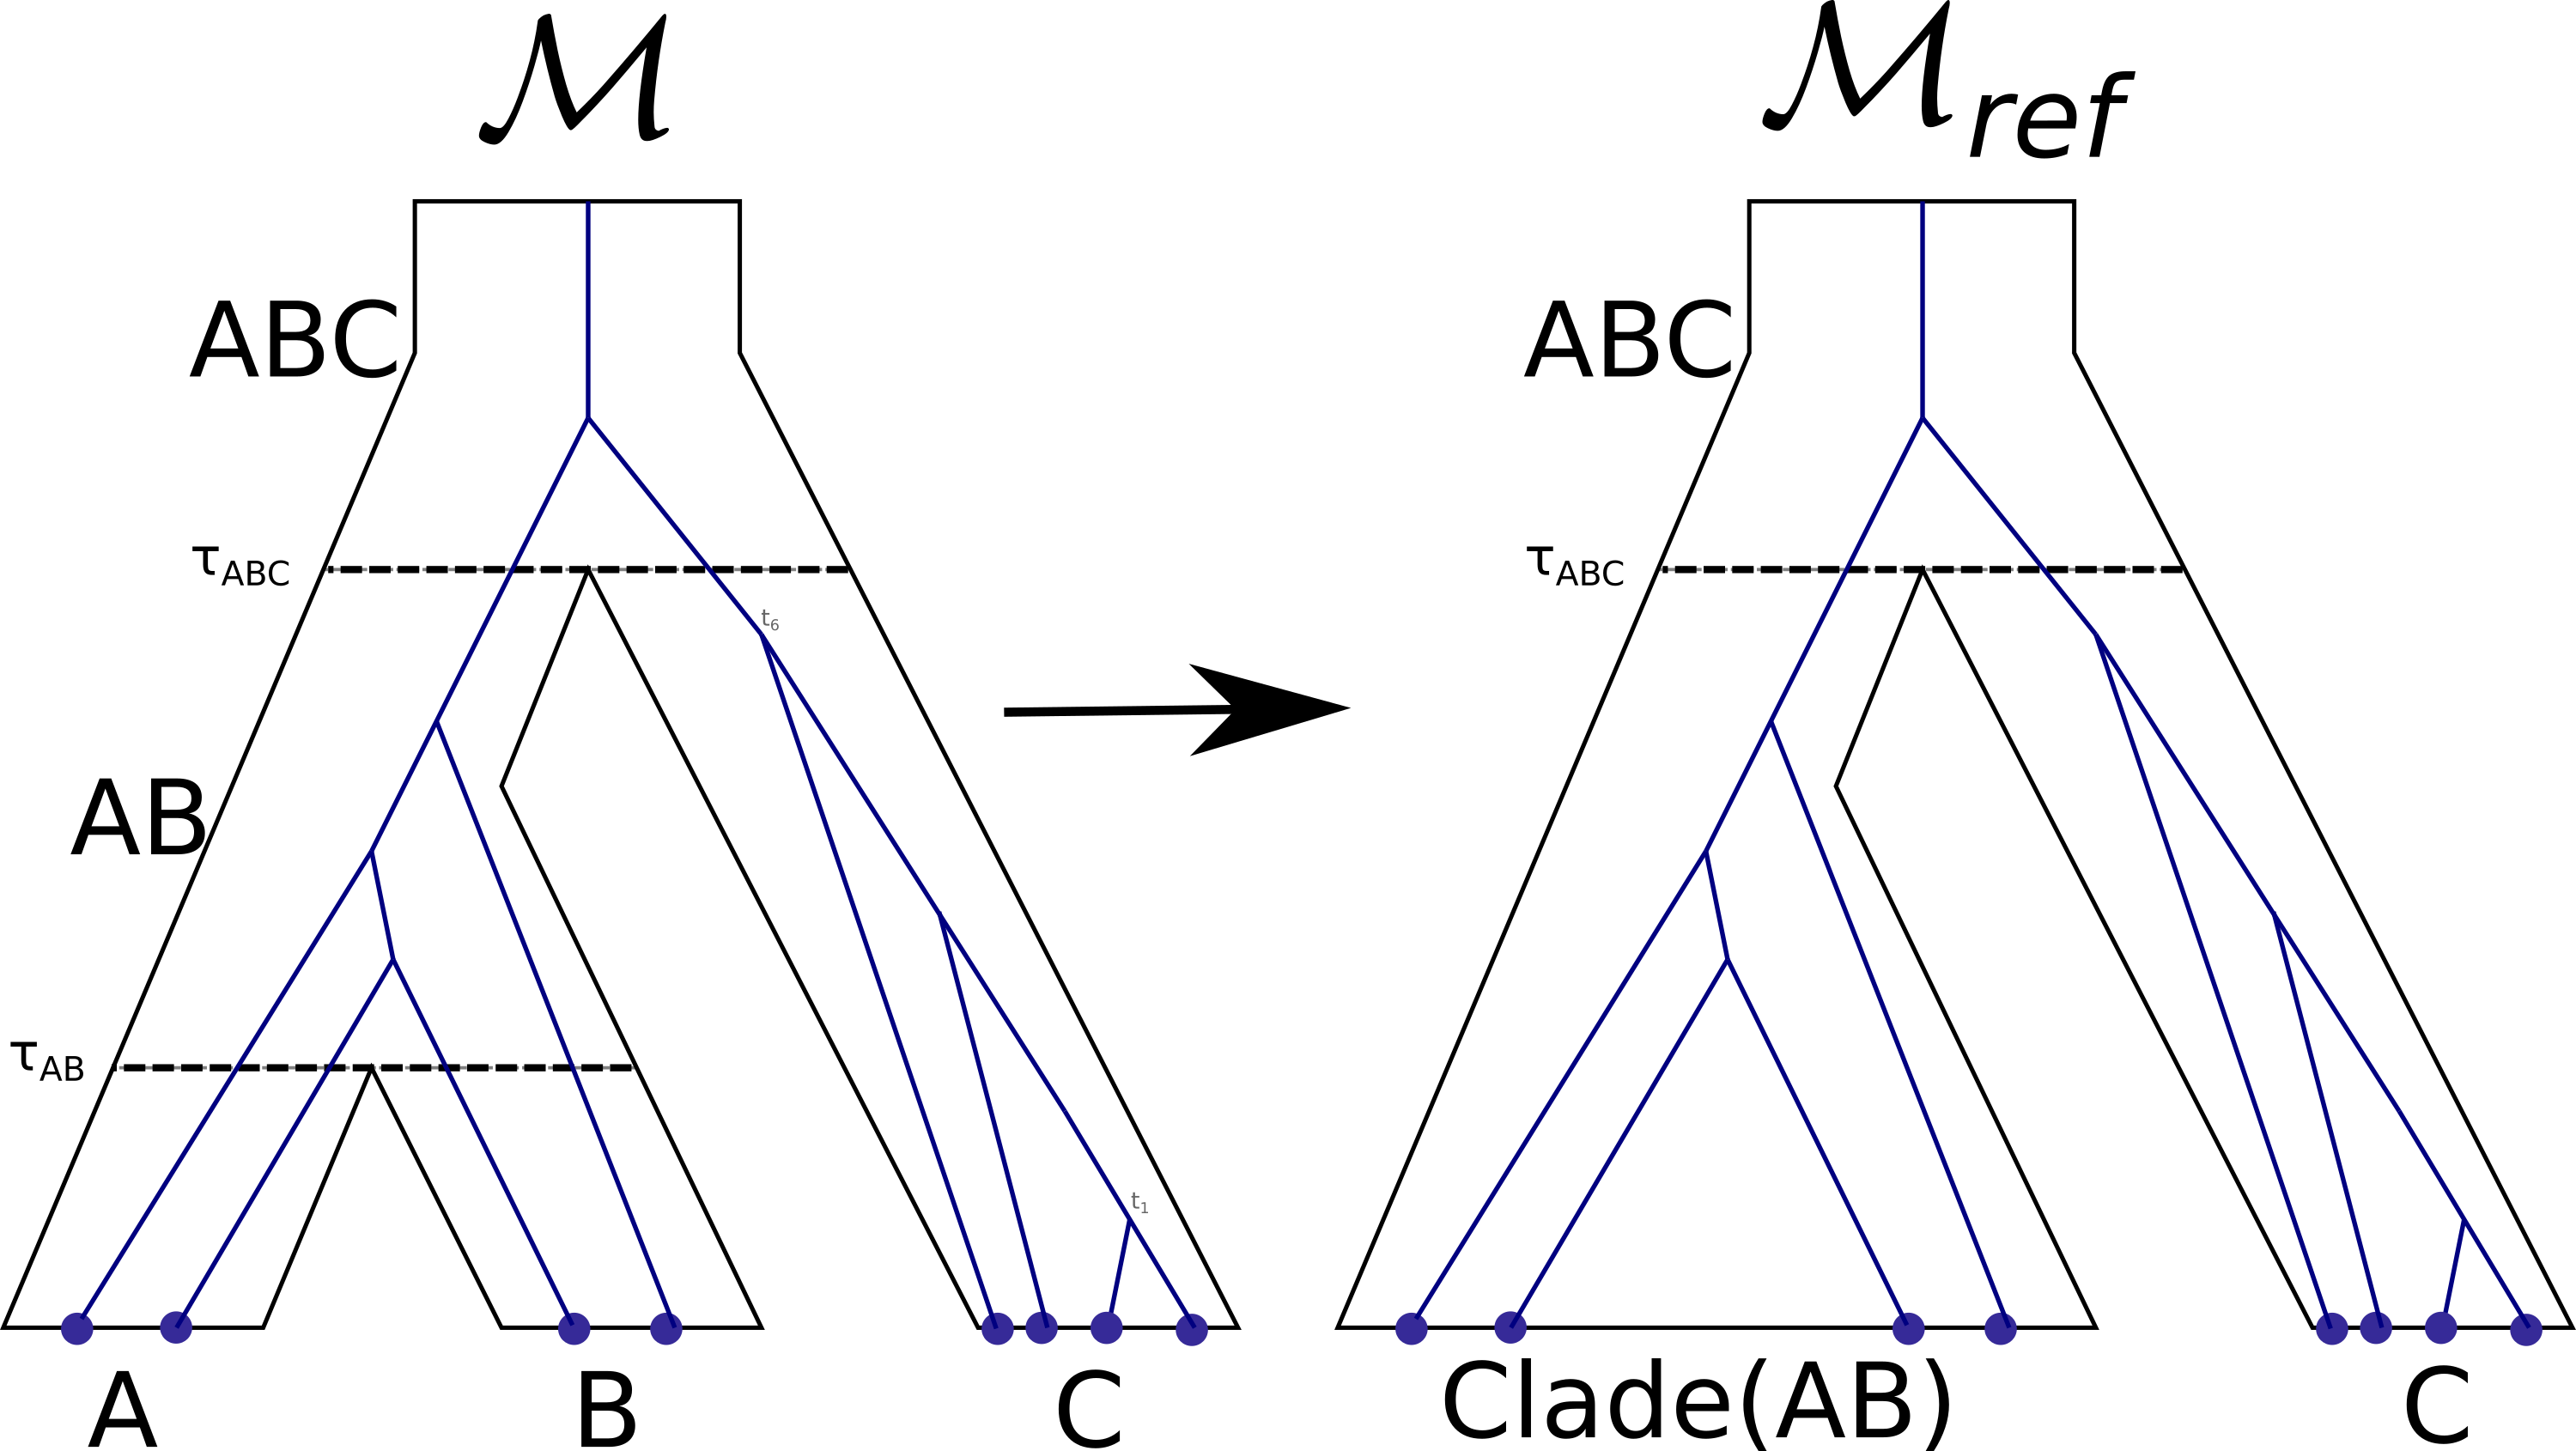
\includegraphics[width=0.8\textwidth]
{clade_collapse_AB}
\caption{\textbf{Construction of a reference model via clade-collapse - } The reference model  $\Mref$ is created by clade-collapsing  the subtree rooted at $AB$ and identically mapping the rest of the hypothesis. When calculating genealogy likelihood over the reference model, we reuse statistics calculated by \gp for $ABC$ and $C$, and need only recalculate genealogy likelihood inside $clade(AB)$. This saves valuable effort in calculation of $P(\G|\T,\Mref)$}
\label{fig:clade_collapse_AB}
\end{figure}


\subsection{Efficient Sufficient Statistics for Reference Model Genealogy Likelihood}


We note that there exists a natural trade-off between the flexibility in choice of reference model and the amount of data the MCMC process is required to emit. For example, if no flexibility is required and the reference model is predetermined before MCMC execution, formula (9) can be calculated during MCMC iteration and only the final RBF value need be emitted. However, calculating (9) on any other reference model would require another full MCMC run.
%
On the other hand, the RBF for every reference model can be computed in post-processing if the MCMC prints out the full hidden state $\GT$ in each iteration.
%
However this would yield an unreasonable amount of traced information, in proportion to the size of the model and to the number of loci.


We designed a computational scheme that aims to find a reasonable middle ground between these two extreme options.
Our objective was to maximize the number of reference models we could consider after running a single MCMC sampling chain without blowing up the output trace.
This is done by identifying a collection of sufficient statistics for $\G$ that satisfy two conditions:
%
%
\begin{enumerate}
 \item The number of sufficient statistics depends on the complexity of the target model, $\Mref$, but not on the size of the data (i.e. the number of individuals and the number of loci).
 \item The sufficient statistics allow calculation of $P(\G|\T,\Mref)$ for a wide variety of reference models and values of model parameters (namely, migration rates and population sizes).
\end{enumerate}
%

Sufficient statistics that satisfy these conditions are derived from the expression for the genealogy likelihood $P(\G|\T, \Mref)$ under Kingman's coalescent, which we briefly recall here.
First, because the loci are assumed to be freely recombining, then the local genealogies $\G=(G_1,...G_L)$ are conditionally independent given the model parameters and the likelihood may be expressed as a product of locus-specific likelihoods, $P(G_l|\T,\Mref)$.  Each locus-specific likelihood is a product of exponentially distributed waiting times for coalescent and migration events. The rates of these exponential distributions depend on the model parameters (population sizes and migration rates) as well as the number of lineages considered for coalescence and migration. We thus identify for each population the set of coalescent and migration events that change the number of lineages modeled in that population in $G_l$. Each time interval $I$ between two consecutive events is associated with the following properties:
\begin{itemize}
 \item $t(I)$ -- the elapsed time of the interval.
 \item $n(I)$ -- the number of lineages of $\G_l$ alive during that time in the target population.
 \item $isCoal(I)$ , $isInMig(I)$  -- binary values that indicate whether the event above the interval is a coalescent event or incoming migration event (respectively).
\end{itemize}
%
%
The contribution of population $p$ to $P(G_l|\T,\Mref)$ can then be expressed as a product over the set of relevant time intervals $\Ip$:
%
%
\begin{small}
\begin{align}
f_{coal}(\G_l,p|\T,\Mref) 
& ~\triangleq~ \prod_{I \in \Ip} \left(\frac{2}{\theta_p}\right)^{isCoal(I)} \exp\left(-\frac{2}{\theta_p}{n(I) \choose 2}t(I)\right) ~. %\notag\\
% & ~=~ \left(\frac{2}{\theta_p}\right)^{numCoals(G_l,p)} \exp\left( -\frac{1}{\theta_p} \sum_{I \in \Ip} (n(I)^2-n(I))~t(I) \right) ~.
\label{eqn:ld-coal}
\end{align}
\end{small}
%
%
Similarly, the contribution of migration band $b$ to $P(G_l|\T,\Mref)$ can be expressed as a product over the set of time intervals $\Ib$ defined by events in the target population of the migration band:
%
%
\begin{small}
\begin{equation}
f_{mig}(\G_l,b|\T,\Mref) ~\triangleq~ \prod_{I \in \Ib} m_{b}^{isInMig(I)} ~ \exp \left( - m_b~ n(I)~t(I)\right) ~.
\label{eqn:ld-mig}
\end{equation}
\end{small}
%
%

Using these notations, the genealogy log likelihood can be expressed as follows:
%
%
\begin{small}
\begin{align}
\ln \left( P(\G| \T,\Mref) \right) ~&=~ \ln \left( \prod_{l}  P(G_l| \T,\Mref) \right)  \notag \\ 
%
&=~  \ln \left( ~\prod_{l}  \left( \prod_{p} f_{coal}(\G_l,p|\T,\Mref) ~ \prod_{b} f_{mig}(\G_l,b|\T,\Mref) \right) ~\right) \notag \\ 
%
&=~  \sum_{p}\sum_{l}\ln \left( f_{coal}(\G_l,p|\T,\Mref) \right) ~ + ~ \sum_{b}\sum_{l}\ln \left( f_{mig}(\G_l,b|\T,\Mref) \right)~. 
\label{eqn:ld-details}
\end{align}
\end{small}

The key to likelihood calculation is to sum over the log-likelihood contributions across time intervals and across loci (see figure \ref{fig:multiple_loci}):
%
%
\begin{small}
\begin{align}
\sum_{l}\ln \left( f_{coal}(\G_l,p|\T,\Mref) \right) &=~ %\sum_{l} \sum_{I \in \Ip} \left( isCoal(I)\cdot \ln \left( \frac{2}{\theta_p}\right)~-~\frac{(n(I)^2-n(I))~t(I)}{\theta_p} \right)\notag \\
%&=~ 
\ln\left( \frac{2}{\theta_p}\right) \sum_{l} \sum_{I \in \Ip} isCoal(I)  - \frac{2}{\theta_p} \sum_{l} \sum_{I \in \Ip}{n(I)\choose 2}t(I) ~.
\label{eqn:ld-coal-stats}\\
% &\notag\\
\sum_{l}\ln \left( f_{mig}(\G_l,b|\T,\Mref) \right) &=~ %\sum_{l} \sum_{I \in \Ib} \left( isInMig(I)\cdot \ln\left( m_b\right) ~-~ m_b n(I) t(I) \right) \notag \\
%&=~
\ln\left( m_b\right) \sum_{l} \sum_{I \in \Ip} isInMig(I)  - m_b \sum_{l} \sum_{I \in \Ip}n(I) t(I) ~.
\label{eqn:ld-mig-stats}
\end{align}
\end{small}

Note that the four double sums in these expressions depend on the local genealogies $\G$ and the divergence times $\{\tau_p\}$, but they do not depend on the population size and migration rate parameters. We thus denote these sums respectively as $numCoals(\G,p)$, $coalStats(\G,p)$,  $numMigs(\G,b)$, and $migStats(\G,b)$, and the log-likelihood can be expressed as follows:
%
%
\begin{small}
\begin{align}
\ln \left( P(\G| \T,\Mref) \right) ~=&~ \sum_{p}  \ln\left( \frac{2}{\theta_p}\right)\cdot numCoals(\G,p) - \frac{1}{\theta_p}\cdot coalStats(\G,p) \\
& +~ \sum_{b}  \ln\left( m_b\right)\cdot numMigs(\G,b) - m_b \cdot migStats(\G,b) ~. 
\label{eqn:ld-final}
\end{align}
\end{small}


\begin{figure}[h]
\centering
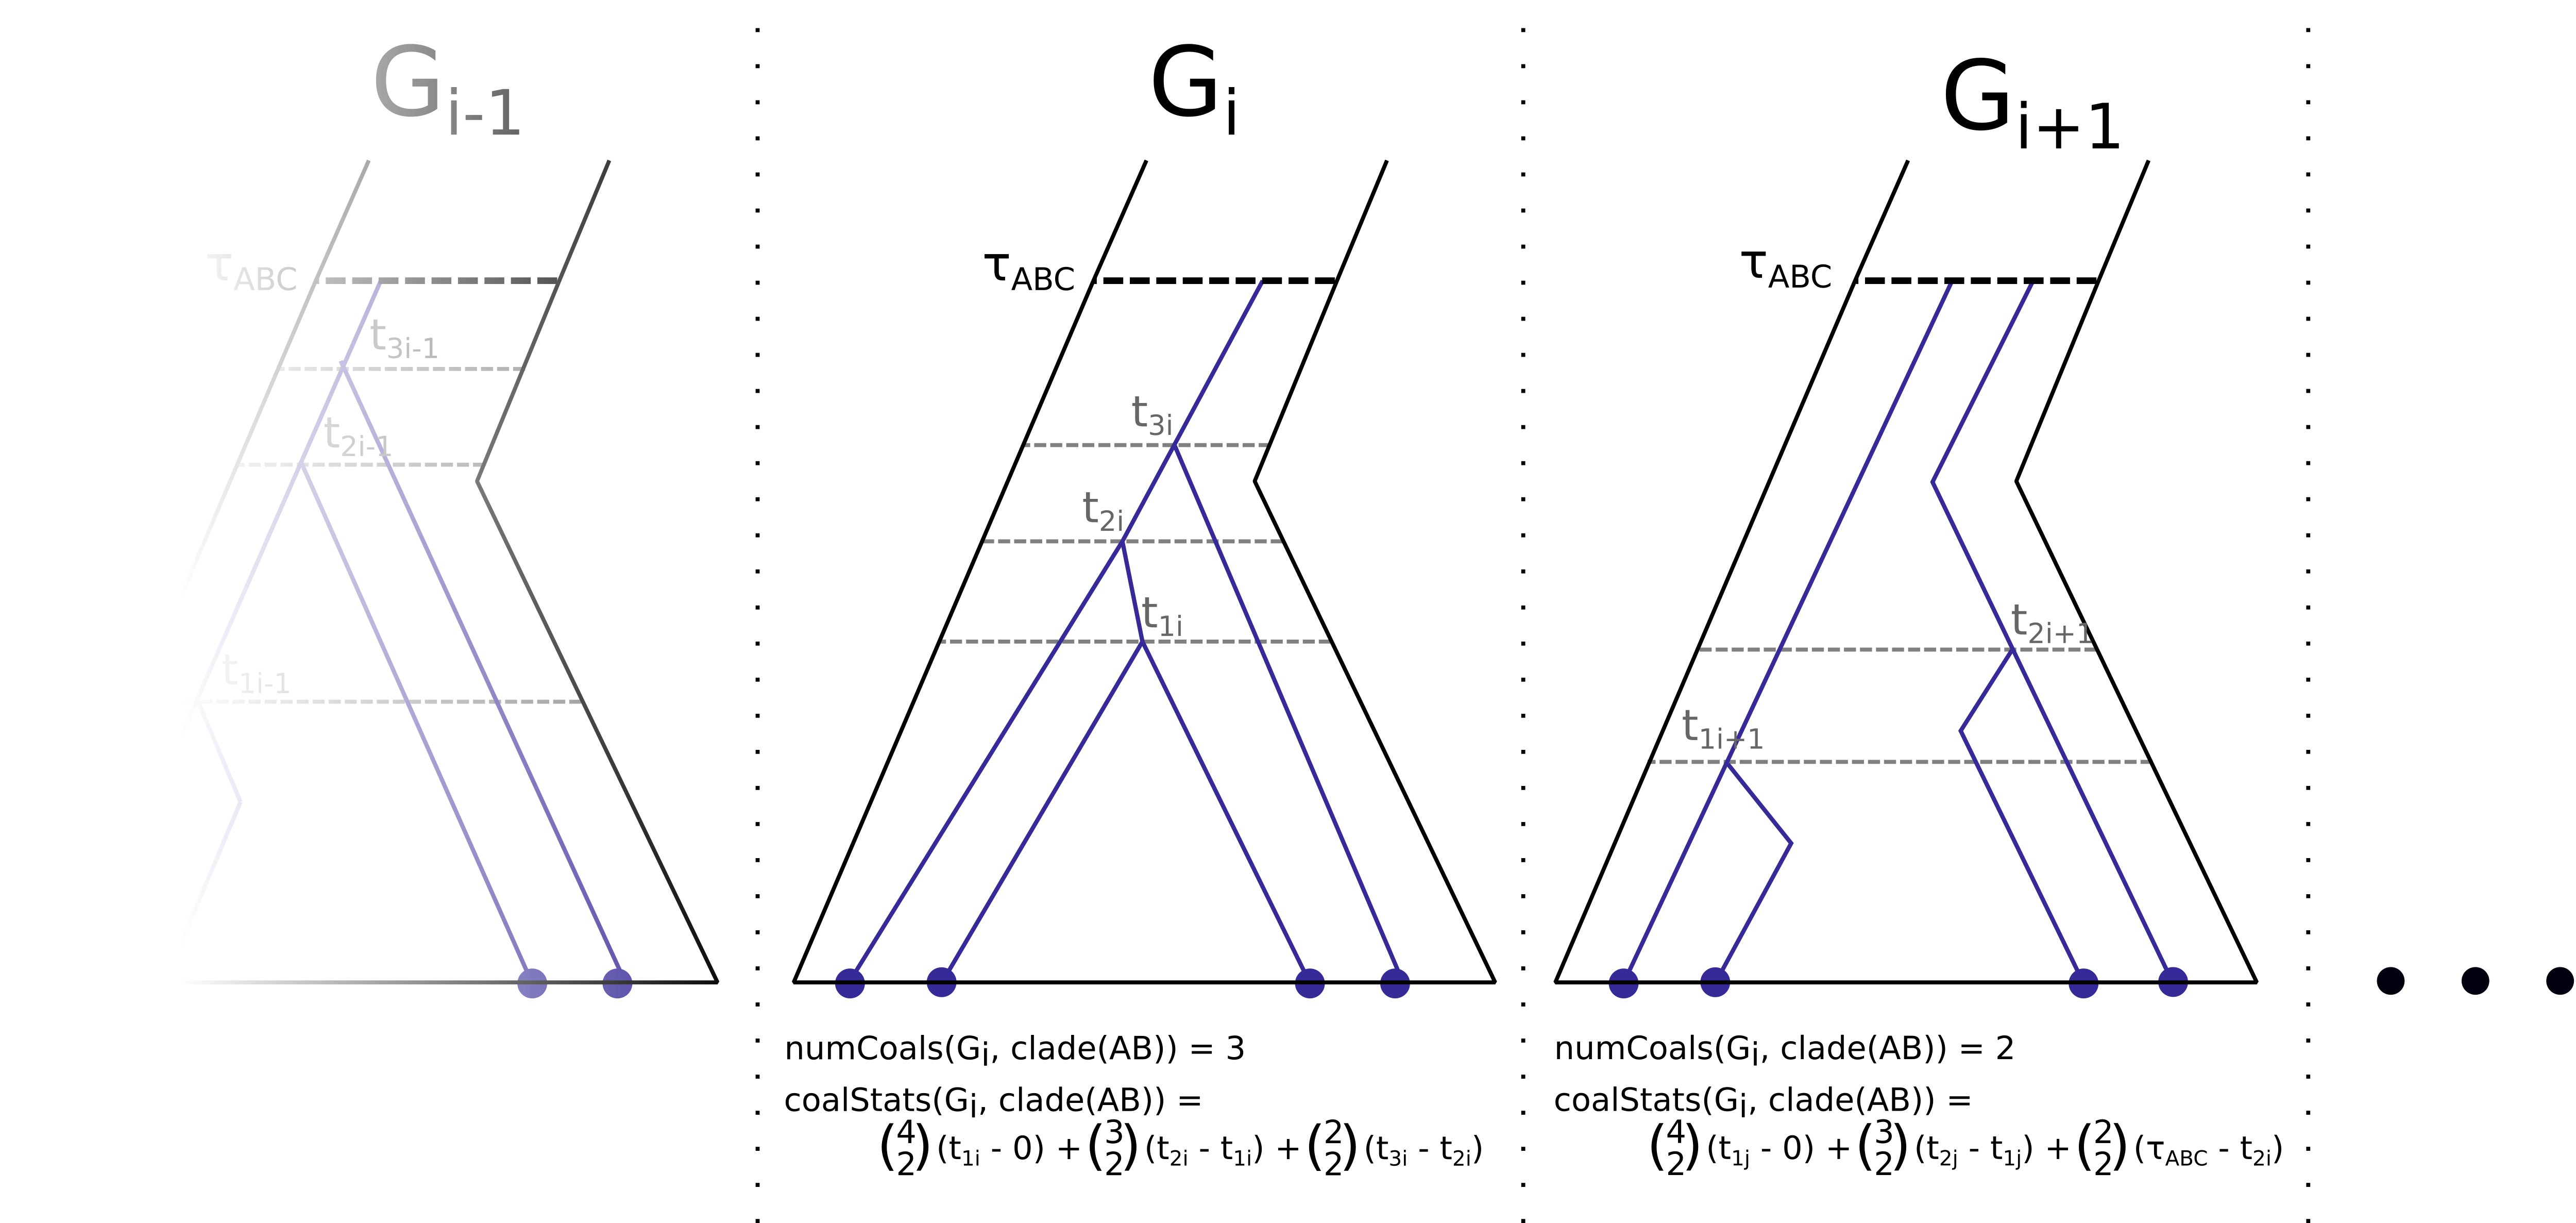
\includegraphics[width=1.0\textwidth]
{multiple_loci}
\caption{The sufficient statistics, \textit{numCoals} \& \textit{coalStats}, are calculated per clade using the time intervals $\Ip$, and are accumulated across loci.\\
%
ALTERNATIVE: The contribution of $clade(AB)$ to $\ln \left( P(\G| \T,\Mref) \right)$ is the sum of it's contributions to the genealogy log-likelihood of all loci. These are calculated for loci $l_i$, using the set of intervals $\mathcal{I}(clade(AB),l_i)$.\\
%
ALTERNATIVE: The sufficient statistic $coalStat(G, clade(AB))$ is calculated by accumulating the Kingman Coalescent genealogy log-likelihod across loci. The contribution of each loci is calculated via the set of intervals $\mathcal{I}(clade(AB),l_i)$. The sufficient statistic $numCoals(G, clade(AB))$ is simply the sum across loci of the amount of coalescnece events inside $clade(AB)$.\\
%
\textcolor{red}{TODO - fix subscript in right genealogy. Also fix fading line above and below left genealogy. Also add another fading genealogy to the right, instead of the dot-dot-dot. Also maybe write somewhere the this is $clade(AB)$}}
\label{fig:multiple_loci}
\end{figure}


The summary statistics $\{~numCoals(\G,p),~~ coalStats(\G,p)~\}_p$~ and ~$\{~numMigs(\G,b),~~ migStats(\G,b)~\}_b$ satisfy our first objective in that their number depends on the complexity of the reference model $\Mref$ but not on the size of the data.
%
They also partly satisfy the second condition, because statistics computed for a given set of local genealogies and given values of divergence times enable computation of the likelihood $P(\G|\T,\Mref)$ for any set of values of the population size and migration rate parameters.
%



\subsection{Recursive Calculation of Sufficient Statistics for Multiple Clade Reference Models}
To support all valid reference models generated by the reference construction process (subsection \ref{Constructing a Reference Model}) we must calculate all summary statistics for every population in every valid reference model.
%
Fortunately, we note that any part of the topology of $\Mref$ which was not transformed during the reference model creation process has the exact same statistics in the $\M$ and in $\Mref$. This allows us to reuse statistics already gathered by \gp for many populations of the reference model. What remain to be calculated are sufficient statistics for all possible clades-  \[\{~numCoals(\G,clade(p)),~~ coalStats(\G,clade(p))~\}_{p\in P_{ref}}\]

To achieve this in an efficient manner, calculation of $numCoals$ and $coalStats$ is done recursively down the population phylogeny of $M$ (see pseudo-python code below). This is done using a function for computing $coalStats$ given a sorted list of intervals (\pythoninline{calculate_coal_stats}), as well as accessors to data from \gp (\pythoninline{num_coals_from_gphocs} \& \pythoninline{sorted_intervals_from_gphocs}):
%

\begin{python}


def recursive_num_coals(pop):
    """recursively calculate and store num of coalescence
    events in clade(pop) as well as all descendant clades"""

    pop_num_coals = num_coals_from_gphocs(pop)

    if is_leaf(pop):
        return pop_num_coals

    left_num_coals = recursive_num_coals(pop.left)
    right_num_coals = recursive_num_coals(pop.right)

    current_num_coals = pop_num_coals + left_num_coals + right_num_coals
    store(current_num_coals)

    return current_num_coals


def recursive_coal_stats(pop):
    """recursively calculate and store coalescence stats
    of clade(pop) as well as all descendant clades"""

    pop_intervals = sorted_intervals_from_gphocs(pop)

    if is_leaf(pop):
        return pop_intervals

    left_intervals = recursive_coal_stats(pop.left)
    right_intervals = recursive_coal_stats(pop.right)
    merged_intervals = merge_sort(left_intervals, right_intervals)

    clade_intervals = merged_intervals.append(pop_intervals)

    clade_coal_stats = calculate_coal_stats(clade_intervals)
    store(clade_coal_stats)

    return clade_intervals

\end{python}

\subsection{Calculating Comb Reference Model Genealogy Likelihood}

Formula \ref{eq:gen_ratio_comb} shows how for a reference model created by comb-collapsing the root population, contribution of the genealogy-likelihood to the model-pairing conditional is reduced to contribution of the portion of genealogies above $\tmin$ - 
\[\frac{ P({\G}_{c|>\tmin}|\M_0,\theta_0=\troot) }{ P(\G_{>\tmin}|\M,\T)} ~ .\]

When comb-collapse is applied to a subtree, we apply the same idea to the portion of the genealogy contained in that subtree. Figure 3 Illustrates the intervals relevant for genealogy-likelihood calculation in the hypothesis and reference models. 


As in the case for clade reference models, we wish to calculate statistics for all viable comb reference models after only one MCMC chain. We do this by storing for every ancestral population $p$ the log of the denominator $~ln(P(\G_{>\tmin}|\M,\T))~$ and the two sufficient statistics involved in the calculation of the enumerator - ($\{~numCoals(\G,comb(p)),~~ coalStats(\G,comb(p))~\}_p$). 
%
This is again calculated recursively down the population phylogeny of $\M$, but the function \pythoninline{calculate_coal_stats} now takes into account only intervals inside the subtree of $p$ and above $\tmin$.


\begin{figure}[h]
\centering
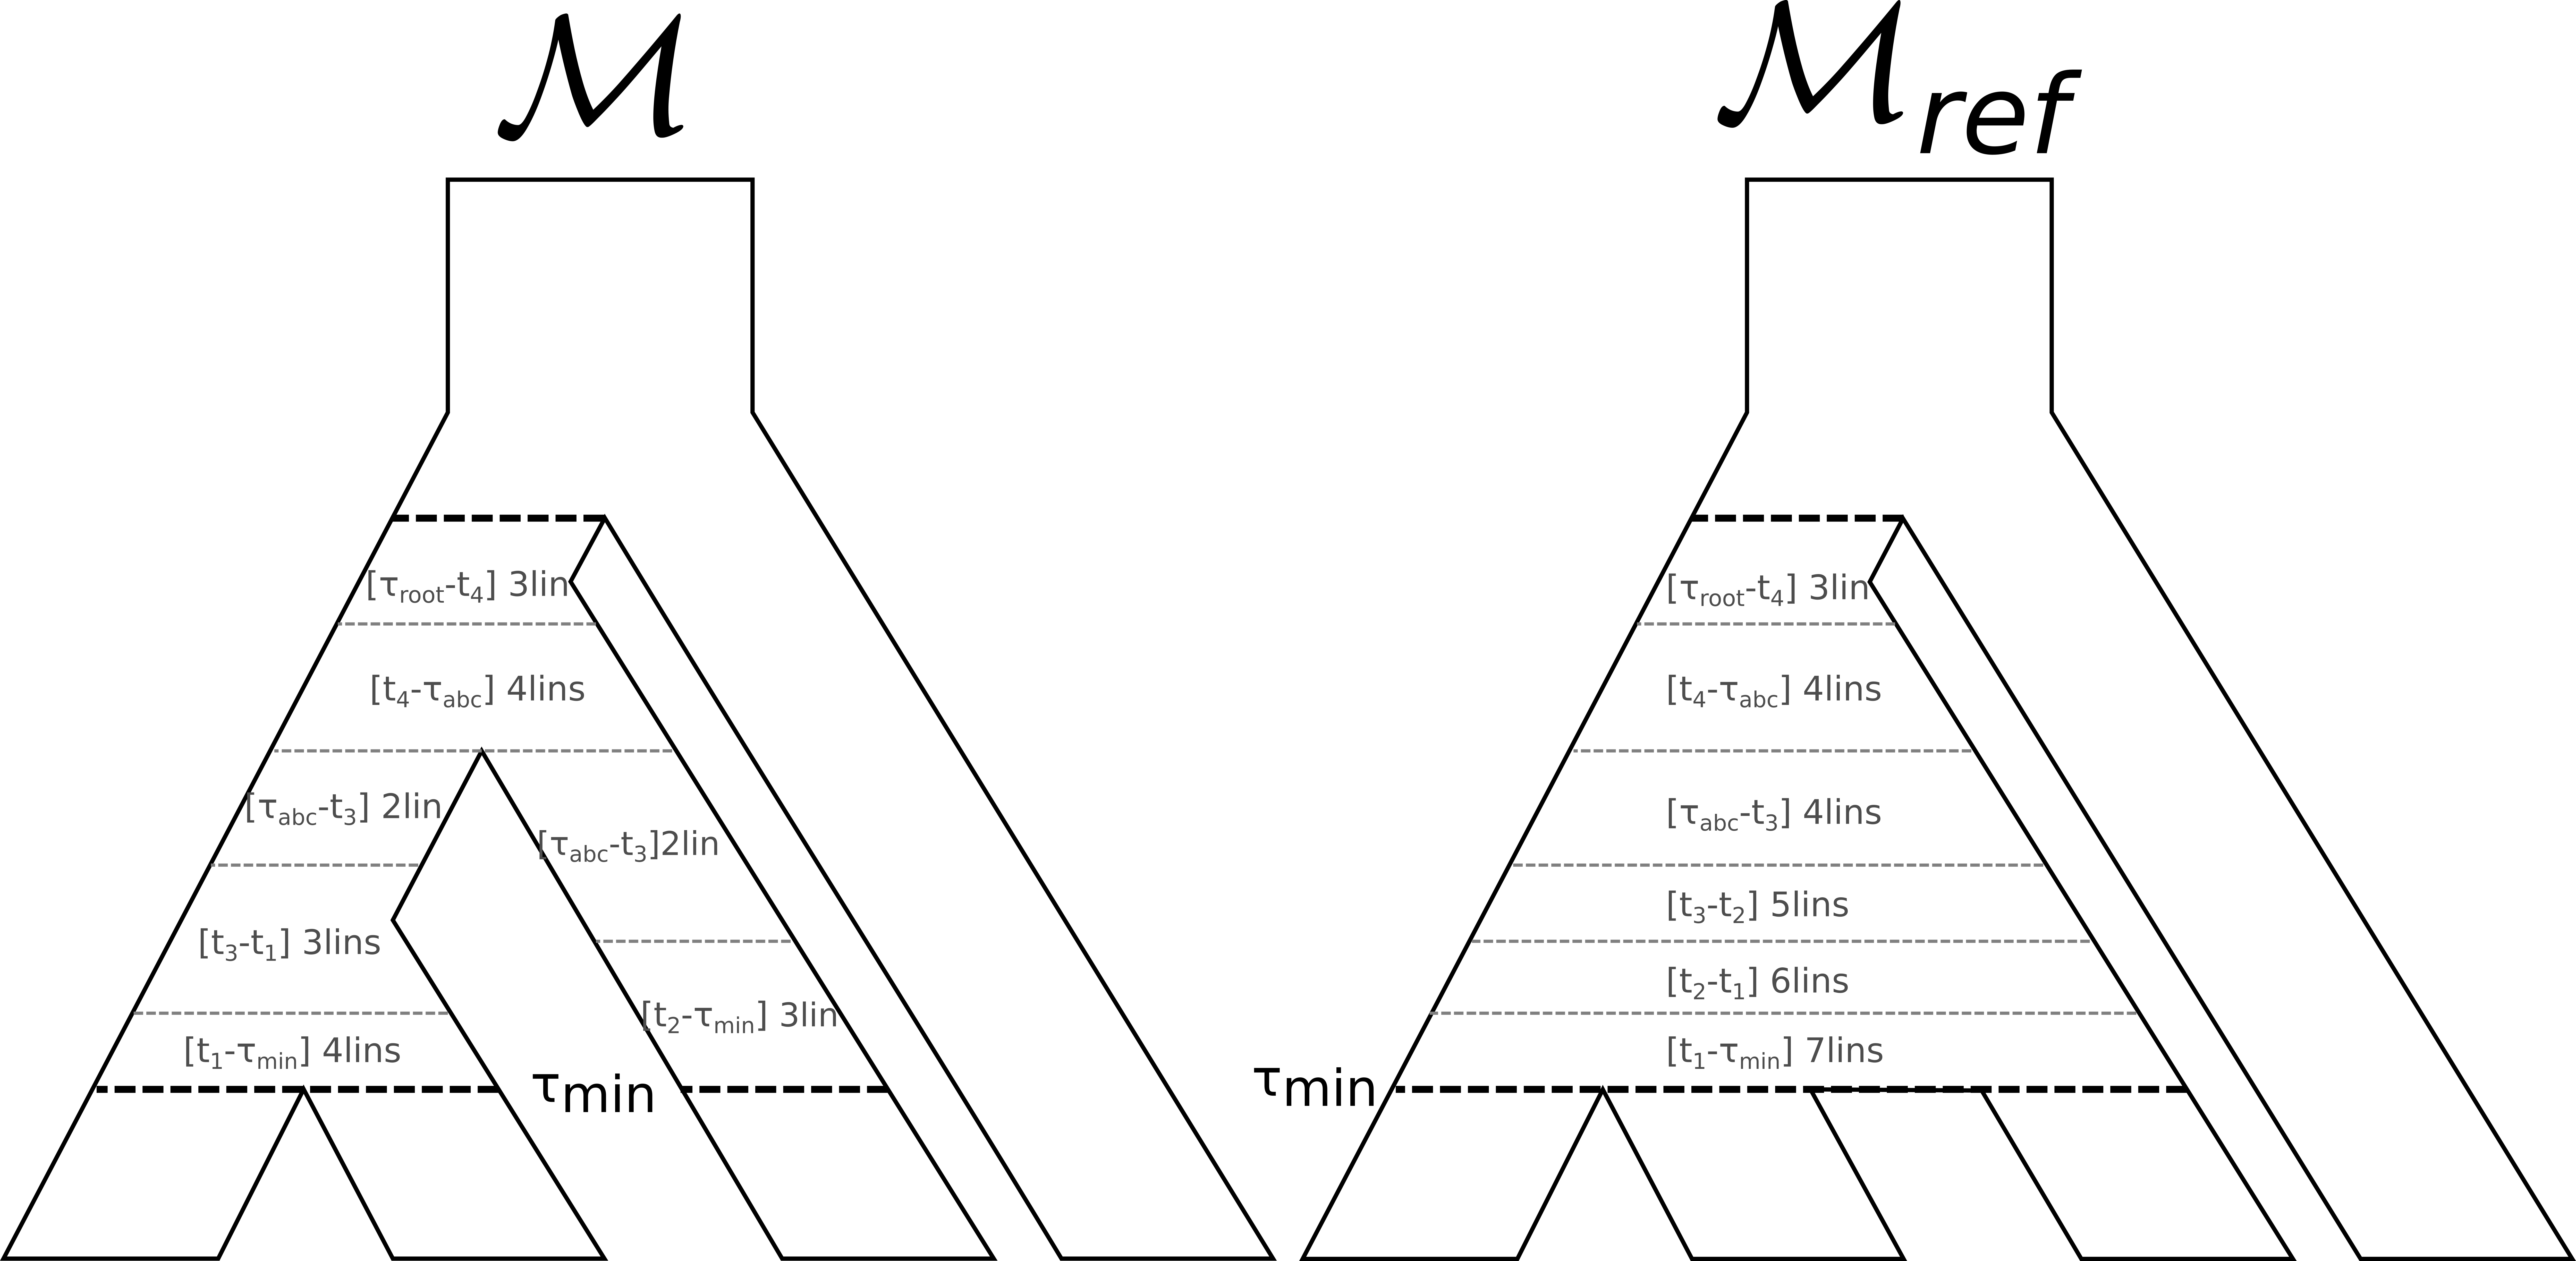
\includegraphics[width=1.0\textwidth]
{hyp_and_comb_intervals}
\caption{In comb reference models, genealogy-likelihood need only be calculated strictly within the bounds of the comb population $comb(p)$. Outside this area of the topology, genealogy-likelihood of the reference and hypothesis models cancels out in the Model-Pairing Conditional. \textcolor{red}{TODO - color the model branches}}
\label{fig:calculate_hyp_stats_above_tmin}
\end{figure}

\newpage
\section{Technicalities and Code}


\subsection{Debugging results}

When examining results of \gp calculations for mcref we were faced with the challenge of validating our results. \#explanation-on-why-this-was-needed. We wished to double-check every statistic emitted, with the simple goal of predictably and reliably reaching our intended calculation.

This was accomplished using a variaty of techniques, restricted by the target statistic and reference model and by the tools at our disposal. 


\begin{itemize}

\item \underline{in comb: compare leaves when comb-age:=inf. Compare root comb when comb-age:=0}

To validate our comb coal-stats calculations we permanantly set the comb-age to various values, allowing us to predict results. When setting a high comb-age (essentially infinite), we asserted That the coal-stats of comb-leaves is equal to the leaf population stats calculated by \gp. When setting comb-age to zero (thus reducing the comb to a clade), we asserted that the coal-stats of the root-comb is equal those of the null reference model (calculated independently by the clade algorithm and by a preexisting \gp implementation).



\item \underline{in clade: compare "leaf clade" with leaf. Compare root-clade with \gp -calculated root-clade}
To assert clade coal-stats, we applied techniques similiar to those used for the comb algorithm. Leaf-rooted clades were compared with leaf stat calculated by \gp and the root-clade (aka the null reference modle) was compared with independantly calculated stats for the null reference model. 

\item \underline{In tau bounds: monotonouty up pop tree. Assert diff(bound, tau) neg correlated with \#loci}

We expected each tau bound to decrease towards its corresponding population tau as the number of loci increases. This due to an increase in the number of coalescence events, leading to an increase in chance of some coalescence event occurring closer to the population tau. We ran a simple set of \gp experiments using the same sequence data, changing only the number of loci in-use. We observed a negative correlation between the number of loci and the tau bound, as expected.

Another simple validation we performed was asserting that bounds are monotonously decreasing down the population tree.

\end{itemize}

\subsection{McRef Code}

\begin{itemize}
\item \underline{configuration}

When setting up mcref, several parameters are configured. The parameters pertain to standard I/O (e.g. where the trace data files are stored and where to store output), to the phylogenic population models (i.e. the structure of the reference and hypothesis models), to \gp configuration (e.g. what alpha \& beta to use for gamma priora, what print multipliers were applied to trace data when emitted by gphocs etc.), to statistical calculations (e.g. how many bootstrap iterations to run during confidence calculation and how much burn-in and sample-skip to use in genealogy likelihood calculation) and to debugging (e.g. what debug calculations to run and visualizations to emit). 

\item \underline{calculating kingman coalescence and kingman migration for the reference model}

Calculating the reference model genealogy likelihood was done using the standard kingman coalescence model, in the same manner implemented in gphocs. The theta of the actual comb/clade population was set to that of the population at the top of the comb/clade and plugged into \#gen\_ld\_ln-formula. 

\item \underline{calculating tau priors for hypothesis and reference models}
tau priors for the hypothesis model were calculated using the same gamma-distribution used by gphocs, based on taus emitted during the \gp run. tau priors for the reference model were calculated using a uniform distribution based on tau-bounds, as described in the chapter about tau bounds.

\item \underline{estimating variance using bootstrap}

In an attempt to estimate the variability of the genealogy likelihood calculation, bootstrap estimations of the rbf were repeatedly sampled from the trace data. 


\item \underline{optimizing runtime (lazily caching trace files, multiprocess concurrently running comparisons, )}

With the goal of optimizing the practical run-time and usability of mcref, several techniques were employed; trace data files, which are repeatedly read and used, are lazily loaded and cached in each mcref process. Multiple mcref experiments are launched using a single command and are cocurrently run in multiple processes, eventually aggregating summary results to a single log file. 

\item \underline{visualizing results}

To clarify results and to help in the understanding and debugging of mcref runs, several visual outputs were developed. each mcref run emits plots of the genealogy-log-likelihood of the reference model and of the hypothesis model, as well as a plot of the rbf calculation across \gp iterations and a plot of the harmonic mean of likelihood of the hypothesis model.

\item \underline{debugging visualizations}

Multiple debug plots are also emitted by mcref. Their goal is to help the researcher assert the experiment was executed as planned. These plots contain the kingman coalescence and kingman migration of every population and migration in both the hypothesis and reference models. They also contain the aggregate coal-stats of the hypothesis and reference model, allowing us to assert that coal-stats of a reference model always exceed those of it's hypothesis \#here-goes-an-explanation-of-the-previous-sentence. 
\end{itemize}



\section{Results}
Results-go-here

\newpage

\section{References}
Bibliography-goes-here

\end{document}
